\subsection{C7 -- Brownian bacteria motion}\label{app:c7}
\paragraph{Native question.} Does the cited recurrent jitter window show the predicted dwell distribution, residual-duration support, cadence-noise band, and service-burden profile?
\paragraph{Native readout.}
\begin{itemize}
\item cited window $\omega_{\mathrm{jit}}$
\item structural key \texttt{tetron:2:2:4}
\item frame count / $T_{\mathrm{eval}}=1024$ bip
\item weighting policy $w(\kappa)\equiv 1$
\item jitter/dwell samples
\end{itemize}
\paragraph{Native operator chain.}
\[
e_\alpha,\ e_\Omega,\ f
\;\to\;
b(\kappa)
\;\to\;
H_B
\;\to\;
B^*
\;\to\;
\Lambda_b
\;\to\;
R_{\mathrm{rest}}
\;\to\;
\text{cadence-noise witness},\ \text{drift witness}.
\]
\paragraph{Native output row.}
\begin{center}
\begin{tabularx}{\linewidth}{@{}lXcclll@{}}
\toprule
Row & Structural key & $B^*$ & $\Lambda_b$ & Dwell distribution & Cadence-noise & Drift \\
\midrule
C7.A & \texttt{tetron:2:2:4} & 2 & 11 & recurrent jitter & jitter band & recurrent \\
\bottomrule
\end{tabularx}
\end{center}
\paragraph{Temporal Conversion Block.} Temporal conversion is a normal chain-rule expansion on the cited native row. This test is retained in native units.
\paragraph{Native figure witness.}
\begin{center}
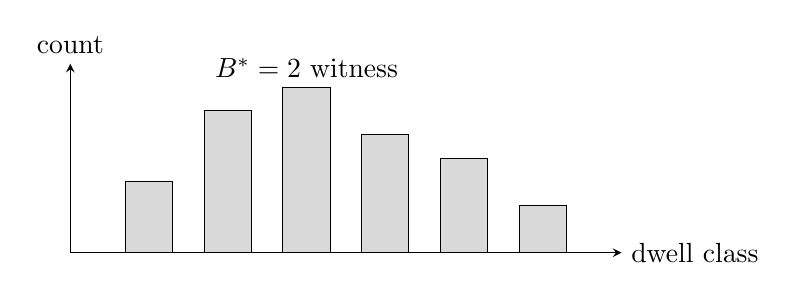
\begin{tikzpicture}[x=1.0cm,y=0.3cm,>=stealth]
\draw[->] (0,0) -- (7,0) node[right] {dwell class};
\draw[->] (0,0) -- (0,8) node[above] {count};
\foreach \x/\h in {1/3,2/6,3/7,4/5,5/4,6/2}{\filldraw[fill=gray!30] (\x-0.3,0) rectangle (\x+0.3,\h);} 
\node[above] at (3,7) {$B^*=2$ witness};
\end{tikzpicture}
\end{center}
\paragraph{Hook / Evidence.} Use the cited recurrent-jitter and dwell-distribution hooks.
